\documentclass[a4paper,11pt]{article}
\usepackage[style=mla,style=authoryear,backend=bibtex]{biblatex}
\renewcommand*{\nameyeardelim}{\addcomma\space}  % add comma between author and year
\setcounter{tocdepth}{2}  % Exclude subsubsections from table of content

\usepackage{graphicx}

% -------- Quoting ------------
\usepackage{mdframed}
\usepackage{xcolor}

\mdfdefinestyle{MyShadeQuoteStyle}{%
    leftmargin=15pt,
    rightmargin=15pt,
    backgroundcolor=gray!25,
    linewidth=0pt,
    skipbelow=\topskip,
    skipabove=\topskip
}

\newenvironment{MyShadequote}[1][]{%
    \ignorespaces%
    \begin{mdframed}[style=MyShadeQuoteStyle,#1]%
}{%
    \end{mdframed}%
    \ignorespacesafterend%
}%
% -------- \Quoting ------------

\addbibresource{bibliography.bib}

\title{Ligeti, Stockhausen and Koenig:\\Aesthetics of Electronic Music}
\author{Tom Gurion}

\begin{document}

\maketitle
\tableofcontents

\section{Introduction and targets}
\label{sec:introduction}

% Citations tests
Ligeti in conversation: (\cite{varnai}).
Stockhausen paper: (\cite{stockhausen}).
Koenig paper: (\cite{koenig})
Ligeti music: (\cite{rami_music}).
Stockhausen music: (\cite{gesang_music}).
Koenig music: (\cite{todo_music}).
Ligeti score: (\cite{rami}).
Stockhausen score: (\cite{gesang}).
The electronic works of Gy{\"o}rgy Ligeti and their influence on his later style: (\cite{levy2006}).

\section{Historical Review}
\label{sec:historical_Review}

Gy{\"o}rgy Ligeti, one of the most innovative musicians of modern 20\textsuperscript{th}-century, was born in Hungary to a Jewish family in 1923.
After suffering from two tyrannies in his youth, Nazi and Stalinist, he left Hungary in 1956 facing western Europe (\cite{ligeti_grove}).
There, he was exposed to electronic music through the Darmstadt-Cologne avant guard ideology, which influenced his writing ever since (\cite[p. TODO]{levy2006}).

Karlheinz Stockhausen, probably the most prominent German composer of the 2\textsuperscript{nd} half of the 20\textsuperscript{th}-century, was born in Cologne in 1928.
He enrolled at the Cologne Musikhochschule in 1947 and graduated in 1951.
After his graduation Stockhausen went to the Darmstadt Internationale Ferienkurse f{\"u}r Neue Musik (the International Summer Courses for New Music) and later moved to Paris, where he met Messiaen, Boulez and Pierre Schaeffer and introduced to the Parisian avant guard and the musique-concr{\`e}te studios.

By 1953 Stockhausen was already established as a leading serialist avant guard composer.
Over the next few years he became the leading figure in Darmstadt-Cologne avant guard scene and from 1956 started to teach regularly at the Darmstadt summer courses (\cite{stockhausen_grove}).

Gottfried Michael Koenig, was born in 1926 in Magdeburg, Germany.
He studied church music in Braunschweig, composition, piano, analysis and acoustics in Detmold, music representation techniques in Cologne and computer technique in Bonn\footnote{Koenig homepage: www.koenigproject.nl/indexe.html}.
During the 1951 Darmstadt summer courses he attended lectures by Meyer-Eppler that awakened his interest in electronic sound production.
In 1953 he moved to Cologne where he studied music technology at the Cologne Hochschule f{\"u}r Music and attended courses on electronic data processing at the University of Cologne.
At the same time he started to work at the studios for electronic music in Cologne, the Nordwest Deutscher Radio (NWDR), first as assistant for other composers and later as a permanent employee and composer (\cite{koenig_grove}).

Darmstadt of post Wold War II became an important center for modern music thereby an attractive place for young composers.
The city is located in the state of Hessen in central Germany, in the American zone of occupation of those days.
The summer courses were financial supported by the US military government with two goals:
first, to propagate American values in effort to reeducate the German population in preparation for the establishment of democratic institutions;
and second, to provide a meeting place where musicians from the former fascist or fascist-occupied areas might further their musical reeducation through exposure to styles and techniques that had been prohibited during the fascist years (\cite{darmstadt_oxford}).
Since the first Darmstadt summer course, in 1948, the focus was on current musical concepts;
at the time it was, mainly, electronic and serail music\footnote{Internationales Musicinstitut Darmstadt: www.internationales-musikinstitut.de/en/summer-course/history/210-history.html}.

In addition to Darmstadt summer courses, the electronic music studios of Cologne were another prominent center for the Darmstadt-Cologne avant guard scene.
The studios were founded in 1951, focused on the creation of pure electronic or ``electroacoustic'' music.
It is believed that the term ``electroacoustic'' was coined by Meyer-Eppler, one of the founders of the studios, to distinguish themselves from musique-concr{\`e}te:
a technique that characterized the already established style of Parisian electronic music (\cite{nwdr}).

The three composers that the current work is about --- Ligeti, Stockhausen and Koenig --- found themselves, each one in its own way, taking part in the Darmstadt-Cologne scene during the 1950\textsuperscript{s}.
Moreover, they all were in a similar stage of their career when they exposed to the ideas presented in the summer courses and the techniques used in the electronic music studios.
These ideas deeply influenced their styles as composers (TODO cite).
However, whereas Stockhausen and Koenig musical styles are direct continuations of these ideas, Ligeti's music cannot be perceived as part of Darmstadt-Cologne style (TODO cite);
his main repertoire is acoustic, and his works are usually not categorized as serial music.

\section{Aesthetic Ideals in Electronic Music}
\label{sec:aesthetic_ideals_in_electronic_music}

In this section I analyze musical concepts as described in \textbf{written materials} by the three composers.
For each composer I analyze one written source:
for Ligeti, I analyze ``Ligeti in conversation'' --- an interview that was conducted by Peter Varnai in 1983 (\citeauthor{varnai});
for Stockhausen, I analyze his 1962 paper ``The concept of unity in electronic music'' (\citeauthor{stockhausen});
and for Koenig, I analyze his 1963 paper ``The Construction of Sound'' (\citeauthor{koenig}).

This work deals with aesthetics of electronic music, hence the decision to choose these papers by Stockhausen and Koenig is trivial.
On the other hand, for Ligeti I choose a source with broader perspective, as his music is usually not categorized as electronic.
Varnai's interview of Ligeti presents a comprehensive set of ideas behind Ligeti's musical style, and I found it useful as a basis to compare the musical concepts with.

Some of the hereby presented concepts are my summaries to the ideas found in the written materials, whereas others are quoted directly from the source.
For those, I add clarification only when absolutely necessary, as I think that most of the concepts are relatively self-explanatory.

Later in this section I will compare these ideas, and search for similarities and differences between them.
A unified understanding of the different ideas by the different composers will be used in the next section to analyze  Ligeti's Ramifications.

\subsection{Ligeti}
\label{sub:eshtetic_ligeti}

The following is a curated list of musical concepts that I have collected from Ligeti's interview.
Ligeti was not listed his concepts explicitly, hence the categorization is done by me and is also subjective.

\subsubsection{Hectic quality / Gesticulation / Deep-frozen expressionism}
\label{subs:ligeti:hectic}

\begin{MyShadequote}
  I want to remove great, whirling passion, all grand expressive gestures, far away and view them at a distance.
  My generation's attitude comes into play here, a rejection of pathos and romanticism (p. 18).
\end{MyShadequote}

\begin{MyShadequote}
  I deprive both pathos and expression of credibility, suddenly everything gets out of gear...
  If pathos in a gesture is excessive you can no longer perceive or register it (p. 19).
\end{MyShadequote}

Indeed, researchers often describe Ligeti's music as pale and nervous dream-like (or even nightmarish) reflection of life.
``Grand emotions are captured in a manner that they do not sound real or believable'' argues Frigyesi, ``gestures exaggerate to the point that it becomes surreal, frightening, absurd, or even comical'' (TODO Frigeyesi).

\subsubsection{Machine like music / Meccanico-type}
\label{subs:ligeti:machine}

\begin{MyShadequote}
  I have always been fascinated by machines that do not work properly...
  Transposed into music, the ticking of malfunctioning machinery occurs in many of my works (p. 16).
\end{MyShadequote}

In addition, researchers pointed out that Ligeti's machines always brake down in his music, what makes them only more frightening (TODO cite).

\subsubsection{Micropolyphony}
\label{subs:ligeti:micropolyphony}

\begin{MyShadequote}
  Both Atmospheres and Lontano have a dense canonic structure.
  But you cannot actually hear the polyphony, the canon.
  You hear a kind of impenetrable texture, something like a very densely woven cobweb.
  I have retained melodic lines in the process of composition, they are governed by rules as strict as Palestrina’s or those of the Flemish school...
  The polyphony structure does not come through, you cannot hear it; it remains hidden in a microscopic, under-water world, to us inaudible (p. 14-15).
\end{MyShadequote}

\subsubsection{Flexible rhythm}
\label{subs:ligeti:flexible}

\begin{MyShadequote}
  What really interested me was flexible rhythm, giving up the pulsating metrical idiom (p. 36).
\end{MyShadequote}

\begin{MyShadequote}
  I built the rhythmic shifts into the music.
  For instance, twenty-four violins would play the same tune but with a slight time-lag between them...
  No violinist can play them, all of them make mistakes, different mistakes all the time.
  These mistakes add up and create a floating, fluctuating patterns (p. 40).
\end{MyShadequote}

\begin{MyShadequote}
  At the time I was interested in the idea of multilayered structures, polyrhythm, and beyond that different tempi, different speed all simultaneously executed (p. 62).
\end{MyShadequote}

\subsubsection{Overwriting / Misleading notation}
\label{subs:ligeti:overwriting}

\begin{MyShadequote}
  My reason for so `overwriting' the score was to achieve the effect I wanted, a sense of danger (p.53).
\end{MyShadequote}

\begin{MyShadequote}
  In a later piece, Ramifications, I divided the strings into two groups with quarter-tone difference in the intonation between them.
  This did not produce music based on quarter-tones; that was not my intention...
  The point is that as the two groups of strings, deliberately tuned apart from one another, go on playing the group tuned higher automatically slides downwards so that the two groups get nearer one another in pitch.
  That is what I wanted: not music based on quarter-tones but mistuned music (p. 54).
\end{MyShadequote}

\begin{MyShadequote}
  ...There will be hardly any difference between various performances; the smudginess both in intonation and in rhythm gives the same result, the same degree of ‘dirtiness’ (p. 55).
\end{MyShadequote}

\begin{MyShadequote}
  ...The passages written in small notes simply indicates that the player should execute them as fast as he can.
  That is why I said that the instrumentalist were not given much freedom; what I kept under control was the overall sound texture at any one time (p. 63).
\end{MyShadequote}

See also the 2\textsuperscript{nd} quote from last subsection (Flexible rhythm -- \ref{subs:ligeti:flexible}).

\subsubsection{``Mistiness'' to ``clearing-up'' process}
\label{subs:ligeti:mistiness}

\begin{MyShadequote}
  My idea was that instead of tension-resolution, dissonance-consonance, dominant-tonic, pairs of opposition in traditional tonal music, I would contrast ``mistiness'' with passages of ``clearing-up''. ``Mistiness'' usually means a contrapuntal texture, a micropolyphonic cobweb technique; the perfect interval appears in the texture first as a hint and then gradually becomes the dominant feature (p. 60).
\end{MyShadequote}

\subsection{Stockhausen}
\label{sub:eshtetic_stockhausen}

Compared to Ligeti, Stockhausen explicitly count 4 characteristics of electronic compositions.
His paper, ``The Concept of Unity in Electronic Music'' opens as following.

\begin{MyShadequote}
  On several previous occasions, when I have been asked to explain the composition of electronic music, I have described four characteristics that seem important to me for electronic composition as distinguished from the composition of instrumental music:

  \begin{itemize}
    \item The correlation of the coloristic, harmonic-melodic, and metric-rhythmic aspects of composition
    \item The composition and de-composition of timbres
    \item The characteristic differentiation among degrees of intensity
    \item The ordered relationships between sound and noise
  \end{itemize}

  Here, I would like to discuss only the correlation of timbre, pitch, intensity, and duration (p. 39).
\end{MyShadequote}

Stockhausens's paper deals mainly with the 1\textsuperscript{st} point above.
However, I will try to glean additional characteristics of electronic music from the paper as well.

\subsubsection{The correlation of timbre, pitch, intensity, and duration}
\label{subs:stockhausen:time}

Stockhausen classifies different sonic elements as different perceptions of the time domain, thus suggesting a unified time model for electronic music.
Periodic elements of short time intervals are intercepted as pitch, and therefore as the basis for melody and harmony;
Periodic elements of medium time interval are intercepted as tempo and rhythm;
Those of larger time intervals supports the musical structure.
Furthermore, according to Stockhausen these ``time spans'' range across 7 octaves each:
Pitch spread across the 7 octaves of the piano;
Tempo and rhythm range from 1/16 of a second up to 8 seconds;
Lastly, time spans of 8 to 1024 seconds are intercepted as structural building blocks.

Based on the above, Stockhausen approaches electronic music as a tool for total serializm (TODO total serializm reference).
Furthermore, he argues that serializm must exist in electronic composition, inherently.

\subsubsection{Lower level building blocks}
\label{subs:stockhausen:sound}

\begin{MyShadequote}
  A musical composition is no more than a temporal ordering of sound events, just as each sound event in a composition is a temporal ordering of pulses.
  It is only a question of the point at which composition begins:
  in composing for instruments whose sounds are predetermined, a composer need not be concerned with these problems.
  On the other hand, in electronic music, one can either compose each sound directly in terms of its wave succession, or, finally, each individual sound wave may be determined in terms of its actual vibration, by an ordering of the succession of pulses (p. 41).
\end{MyShadequote}

\begin{MyShadequote}
  One would not proceed from sound properties that had already been experienced and then allow these to determine temporal variations;
  instead, one would compose the temporal arrangements of pulses themselves, and discover their resultant sound properties experimentally (p. 42).
\end{MyShadequote}

\subsubsection{Noise}
\label{subs:stockhausen:noise}

Stockhausen notes that in traditional instrumental music harmony and melody are always based on whole-number divisions of pitches.
Therefor, ``indicating the necessity of excluding noise from this kind of music'' (\cite[p. 47]{stockhausen}).
This idea shifts naturally to rhythm, and from there, similarly, to form and structure.

Referring back to Stockhausen first concept (in section \ref{subs:stockhausen:time}), a unified model for time in music solves the above by introducing ``noise'' in all different ranges of the time domain -- from timbre to form.

\subsection{Koenig}
\label{sub:eshtetic_koenig}

``The Construction of Sound'' by Koenig (\cite*{koenig}) deals mainly with serial music and in different ways that serial decisions can be incorporated into electronic music.
The current work explores aesthetics in electronic music.
Thus, in this section I try to extract electronic music characteristics from the serial music context in which they are presented in the paper.

\subsubsection{Sounds of unlimited lengths}
\label{subs:koenig:lengths}

\begin{MyShadequote}
  (Intrumental music characterized by) homogeneous, continuous sounds of limited lengths.
  One might say that all classic categories of melodic formation, counterpoint, harmony, form and instrumentation have their origins in this manner of production.
  (On the other hand), the length of electronically produced sound is theoretically unlimited...
  The classic categories thus do not apply to electronic music;
  at any rate they do not have their origins in the new material and the way in which it is produced (p. 1-2).
\end{MyShadequote}

\subsubsection{Non-stationary sounds}
\label{subs:koenig:nonstationary}

Koenig classify timbre into ``classes''.
Both instrumental and electronic music share three classes of continuous sounds:
Harmonic sound, which consists a fundamental; Noise sound, without fundamental; and impulses, which have no timbre nor fundamental.
According to Koenig ``(for the three classes above) we have one timbre for each attack'' (p. 17).

Electronic music enhances the timbre possibilities with another class:

\begin{MyShadequote}
 Electronic music also knows a family of non-stationary sounds with a duration, but no constant timbre...
 Since their ``timbre'' is not constant, it can be described but not accurately imagined.
 The movement of the timbre rather follows the compositional process of the micro-time range.
 In this ways structures are composed instead of timbre (p. 18).
\end{MyShadequote}

\subsubsection{Sound as a formal event}
\label{subs:koenig:event}

\begin{MyShadequote}
  The electronically produced sound does not have to be homogeneous and continuous.
  One complete sound can consist of several individual components whose determinants may change in the next sound.
  The sound is a closed unit and becomes a means of formation;
  each sound characteristic becomes a formal event.
  Instrumental music composes ``with'' sounds, electronic music composes sounds (p. 2).
\end{MyShadequote}

\subsubsection{Representation of pitch ranges}
\label{subs:koenig:pitch_ranges}

This paper deals mainly with serializm, and how it is applied to electronic music.
The following idea came from this way of thinking, in serias, but I believe that it might by understood and analyzed even without considering serial decisions.
Here, Koenig describe different ways to represent a pitch range.

\begin{MyShadequote}
  \begin{description}
    \item[Pointillistically] - single pitches are used in such a way that the limits of the range are frequently touched.

    \item[In planes] - the range is filled as continuously as possible...
    The range as a whole is clear, since limits and interior are uniformly occupied.

    \item[Articulated in planes] - the entire plane of the range is divided up into changing sections which in their turn can be either pointillist or planes:
    pointillist as ``chords'', clusters of various sizes;
    planes in the form of smaller planes within the larger one.

    \item[Transition] - it is a simple matter to have a regular transition from planes to points if the plane is brought about by a rapid sequence of points by:
    (a) slowing down the process,
    or (b) reducing the number of layers step by step (p. 11).
  \end{description}

\end{MyShadequote}

\subsection{Comparison}

\begin{figure}[!htb]
  \centering
  \textbf{Categorization of ideas}\par\medskip
  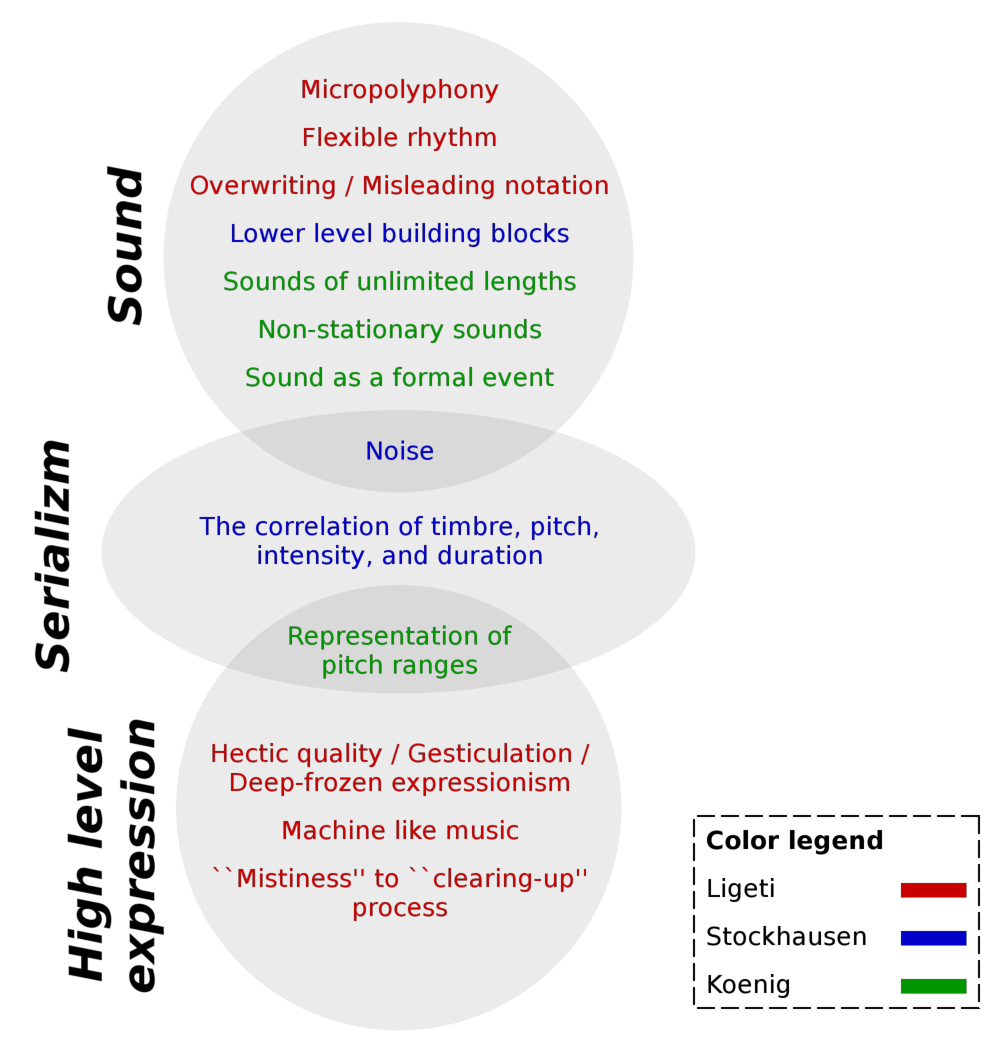
\includegraphics[width=\linewidth]{graphics/concepts_categorization.pdf}
  \caption{Subjective categorization of ideas to sound, serializm and high level expressions.}
  \label{fig:concepts_categorization}
\end{figure}

TODO regarding the first concept by Stockhausen:
Overall, I can not find a common ground between this compository element to those of Ligeti that were mentioned before.
Their attitudes regarding unified perception of time are, most probably, contradicting.

TODO regarding the 2nd concept by stockhausen:
Ligeti also refer to this ideas:

\begin{MyShadequote}
  Modification of timbre and dynamics are obviously very significant but the patterns emerging from them are even more important...
  I should say that the changes and modifications of the overall pattern are the important feature, not the tone colors. (Ligeti in conversation, p. 39).
\end{MyShadequote}

\section{Ligeti's Remifications}
\label{sub:ramifications}

Ligeti ideals and characteristics as found in Remifications.

\subsection*{Micropolyphony, flexible rhythm and misleading notation}

This ideas are perhaps the most dominants in this composition.
Examples can be found in the 0:00 - 1:55, 4:20 - 4:35, 5:28 - 6:25.

\subsection*{Machine like music / Meccanico-type}

It appears to me that these idea could be counted together with the previous ones.
On the other hand, some parts in Remifications are dominated by more ``machine-like'' characteristics than others.
For example: 5:28 - 6:25, 7:00 - 8:00.

\subsection*{Hectic quality / Gesticulation / Deep-frozen expressionism}

Gesticulated phrases appears in Remifications only for short periods, they are not characterize the composition as a hole.
Nevertheless, we can note two ``overly exaggerated'' phrases, where the primer is a bit more distinct in that manner: 3:36 - 3:45, 6:28 - 6:40.
One could argue that these are just dramatic phrases within the composition, but I suspect that this amount of vibrato in Ligeti's composition most present some decent amount of cynicism.
TODO cite frigyesi to support this statement.

\subsection*{‘Mistiness’ to ‘clearing-up’ process}

In my opinion this idea is the lessen distinct in this composition.
This is probably because of the firm voice that accompanies any of the mictrotonal parts, while the ``mistiness'' microtonal is steady and is not ``clearing-up'' into an perfect interval.
The most relevant parts I managed to find for this idea are: 1:40 - 2:08, 2:19 - 2:38.

\section{General Discussion}
\label{sec:general_discussion}

\printbibliography[title={Bibliography}]

\end{document}
